\documentclass[]{ktu}
\usepackage{times}

\begin{document}
\renewcommand{\listfigurename}{Paveikslų sąrašas}

\thispagestyle{noNumber}
\begin{center}

\includegraphics[width=2.46cm]{ktu.pdf}
\vspace{0.3cm}

\normalsize{\textbf{Kauno technologijos universitetas}} \\
Informatikos fakultetas

\vspace{5cm}

\Large \textbf{Projekto pavadinimas} \\
\large
Baigiamasis bakalauro projektas

\vspace{3cm}

\normalsize
{\color{lines_name} \line(1,0){180}}\\
\vspace{0.5cm}
\textbf{Vardenis Pavardenis} \\
Projekto autorius

\vspace{1cm}

\textbf{doc. dr. Vardenis Pavardenis} \\
Vadovas\\
\vspace{0.5cm}
{\color{lines_name} \line(1,0){180}}\\
\vfill

\textbf{Kaunas, 2024}

\end{center}

\thispagestyle{noNumber}
\begin{center}

\includegraphics[width=2.46cm]{ktu.pdf}
\vspace{0.3cm}

\normalsize{\textbf{Kauno technologijos universitetas}} \\
Informatikos fakultetas

\vspace{5cm}

\Large \textbf{Projekto pavadinimas} \\
\large
Baigiamasis bakalauro projektas\\
\vspace{0.1cm}
Dirbtinis intelektas (6121BX035)
\vspace{3cm}
\begin{flushright}
\begin{minipage}{7cm}
{\color{lines_name} \line(1,0){180}}\\
\normalsize{\textbf{Vardenis Pavardenis}} \\
\normalsize{Projekto autorius}\bigskip \\ %
\normalsize{\textbf{doc. dr. Vardenis Pavardenis}} \\
\normalsize{Vadovas} \bigskip \\ 
\normalsize{\textbf{jaun. asist. V. Pavardenis}} \\
\normalsize{Recenzentas} \\
{\color{lines_name} \line(1,0){180}}\\
\end{minipage}
\end{flushright}
\vfill

\normalsize{\textbf{Kaunas, 2024}}
\end{center}

\thispagestyle{noNumber}
\begin{center}

\includegraphics[width=2.46cm]{ktu.pdf}
\vspace{0.3cm}

\normalsize{\textbf{Kauno technologijos universitetas}} \\
Informatikos fakultetas \\
Vardenis Pavardenis

\vspace{3cm}

\Large \textbf{Project Name} \\
\large
Akademinio sąžiningumo deklaracija

\vspace{1cm}
\end{center}

Patvirtinu, kad:
\begin{enumerate}
\item{
        baigiamąjį projektą parengiau savarankiškai ir sąžiningai,
        nepažeisdama(s) kitų asmenų autoriaus ar kitų teisių, laikydamasi(s)
        Lietuvos Respublikos autorių teisių ir gretutinių teisių įstatymo
        nuostatų, Kauno technologijos universiteto (toliau – Universitetas)
        intelektinės nuosavybės valdymo ir perdavimo nuostatų bei Universiteto
        akademinės etikos kodekse nustatytų etikos reikalavimų;
}
\item{
      baigiamajame projekte visi pateikti duomenys ir tyrimų rezultatai yra
      teisingi ir gauti teisėtai, nei viena šio projekto dalis nėra plagijuota
      nuo jokių spausdintinių ar elektroninių šaltinių, visos baigiamojo
      projekto tekste pateiktos citatos ir nuorodos yra nurodytos literatūros
      sąraše;
}
\item{
      įstatymų nenumatytų piniginių sumų už baigiamąjį projektą ar jo dalis niekam nesu mokėjęs (-usi);
}
\item{
      suprantu, kad išaiškėjus nesąžiningumo ar kitų asmenų teisių pažeidimo
      faktui, man bus taikomos akademinės nuobaudos pagal Universitete
      galiojančią tvarką ir būsiu pašalinta(s) iš Universiteto, o baigiamasis
      projektas gali būti pateiktas Akademinės etikos ir procedūrų
      kontrolieriaus tarnybai nagrinėjant galimą akademinės etikos pažeidimą.
}

\vspace{2cm}
\begin{flushright}
\begin{minipage}{5cm}
Vardenis Pavardenis \\
\textit{Patvirtinta elektroniniu būdu}
\end{minipage}
\end{flushright}

\end{enumerate}

\thispagestyle{noNumber}
Vardenis Pavardenis. Projekto pavadinimas.
Bakalauro studijų baigiamasis projektas / vadovė doc. dr. Vardenis Pavardenis; Kauno technologijos universitetas, Informatikos
fakultetas.

Studijų kryptis ir sritis (studijų krypčių grupė): Informatika (Informatikos mokslai).

Reikšminiai žodžiai: informacinė sistema, LaTeX.

Kaunas, 2024. 60 p.
\section*{Santrauka}
Lorem ipsum dolor sit amet, eam ex decore persequeris, sit at illud lobortis
atomorum. Sed dolorem quaerendum ne, prompta instructior ne pri. Et mel
partiendo suscipiantur, docendi abhorreant ea sit. Recteque imperdiet eum te.
Eu eum decore inimicus consetetur, cu usu habeo corpora intellegam. Ut antiopam
efficiendi deterruisset sit. Mel sint eirmod id, qui quot virtute id, dolor
nemore forensibus usu id. Fugit dolore voluptatum cu vim. An vix veniam graecis
insolens, sit posse iusto id. Ut vim ceteros percipit, id quo ubique recusabo,
eum sint lucilius ea. In sumo inani numquam has.

\pagebreak

\thispagestyle{noNumber}
\pagebreak
Vardenis Pavardenis. Project name.
Bachelor's Final Degree Project /
supervisor assoc. prof. Vardenis Pavardenis. Faculty of Informatics, Kaunas University of Technology.

Study field and area (study field group): Informatics (Computing).

Keywords: system, LaTeX.

Kaunas, 2024. 60 pages.
\section*{Summary}
Lorem ipsum dolor sit amet, eam ex decore persequeris, sit at illud lobortis
atomorum. Sed dolorem quaerendum ne, prompta instructior ne pri. Et mel
partiendo suscipiantur, docendi abhorreant ea sit. Recteque imperdiet eum te.
Eu eum decore inimicus consetetur, cu usu habeo corpora intellegam. Ut antiopam
efficiendi deterruisset sit. Mel sint eirmod id, qui quot virtute id, dolor
nemore forensibus usu id. Fugit dolore voluptatum cu vim. An vix veniam graecis
insolens, sit posse iusto id. Ut vim ceteros percipit, id quo ubique recusabo,
eum sint lucilius ea. In sumo inani numquam has.
\pagebreak

\thispagestyle{noNumber}
\hspace*{-1cm}
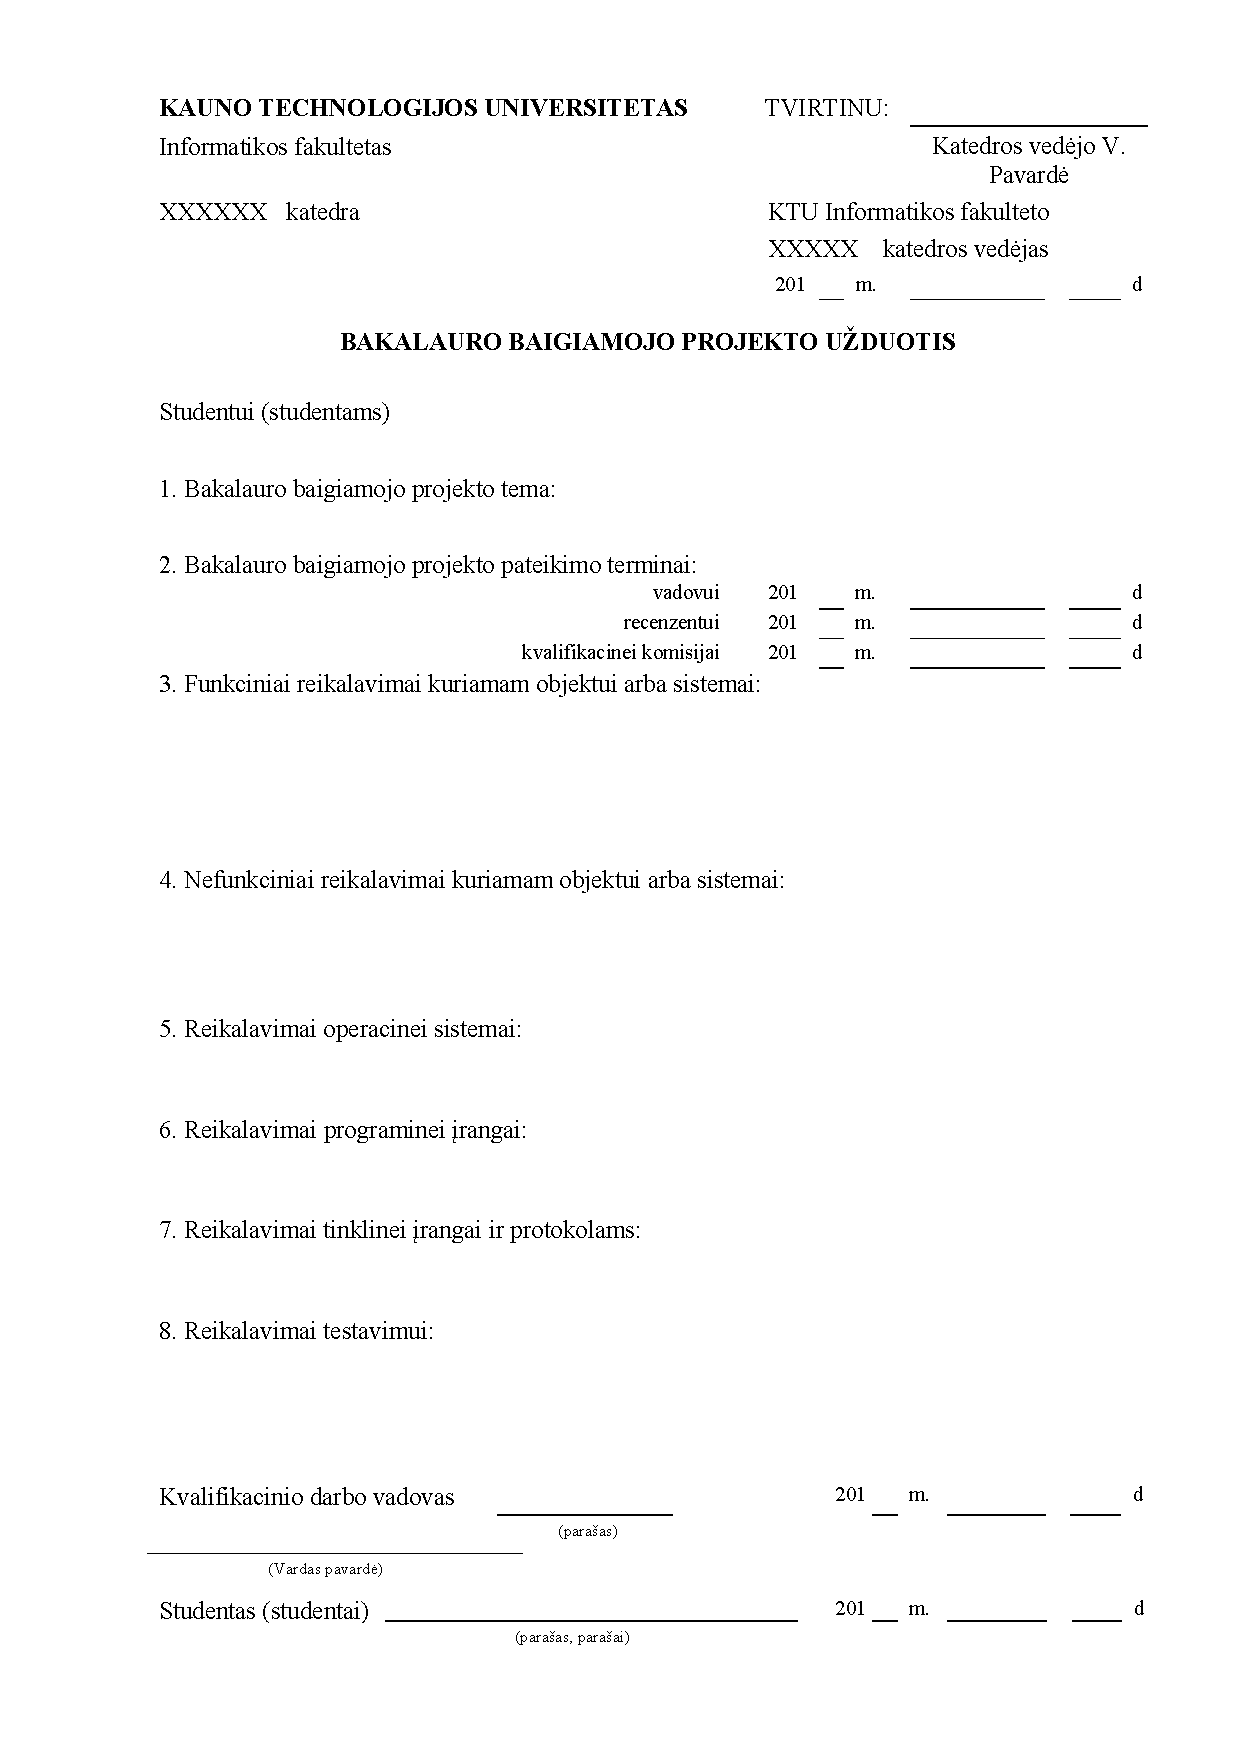
\includegraphics[scale=0.8]{problem_stm.pdf}

\setstretch{1.1} % Jog tilptu viskas viename puslapyje
\tableofcontents
\setstretch{1.15}
\pagebreak
\listoftables
\addcontentsline{toc}{section}{Lentelių sąrašas}
\pagebreak
\listoffigures
\addcontentsline{toc}{section}{Paveikslų sąrašas}
\pagebreak
\section*{Įvadas}
Įvado pradžioje nurodoma, kokiai studijų programai ir specializacijai priklauso
darbas. Dirbtinio intelekto studijų programos studentai specializacijų neturi
(todėl nurodo tik studijų programą), Informatikos studijų programos studentai
nurodo vieną iš trijų variantų: Interneto informatika (specializacija),
Multimedijų sistemos (specializacija), Asmeninis modulių rinkinys. 

Toliau supažindinama su darbo specifika, aktualumu, išdėstomi tikslai bei uždaviniai,
praktinė darbo reikšmė, aptariama dokumento struktūra. Šiame skyriuje apie
darbą kalbama abstrakčiai, nederėtų pateikti nuorodų į kitus šaltinius (1 – 2
lapai). 

\subsection*{Darbo problematika ir aktualumas}
Apibrėžiama darbo problematika ir aptariamas aktualumas. Šiame poskyryje taip pat nurodoma su darbu susijusi sritis, praktinė darbo reikšmė.
\subsection*{Darbo tikslas ir uždaviniai}
Suformuluojamas pagrindinis darbo tikslas, kuris išskaidomas į kelis uždavinius (3 – 6 uždaviniai). Išvados dokumento pabaigoje formuluojamos uždavinių pagrindu.
\subsection*{Darbo struktūra}
Aptariama dokumento struktūra. Nurodoma kiek ir kokių skyrių dokumente yra ir kokia informacija juose pateikiama.
\addcontentsline{toc}{section}{Įvadas}

\section{Analizė}
Su darbo problematika susijusios informacijos analizė (8 – 12 lapai). Čia analizuojama kitų autorių literatūra, technologijos, standartai ir įranga: su tematika susijusios literatūros analizė, aktualių technologijų analizė, susijusios programinės ir techninės įrangos analizė, galimybių analizė, situacijos rinkoje analizė ir kt. Analitinė dalis baigiama atliktos analizės išvadomis.
\subsection{Projekto aktualumas} 
\subsection{Konkurentų analizė}
\subsubsection{Vartotojo sąsajos technologijų analizė}
\subsubsection{Serverio technologijų analizė}
\subsubsection{Gilaus mokymo karkasų analizė}
\subsubsection{Duomenų bazės technologijų analizė}

\section{Projektas}
Aprašoma sistemos/įrankio/paslaugos projektavimo stadija, pateikiama detali
specifikacija (8 – 12 lapai). Apibrėžiama kuriamo produkto vizija (koncepcija).
Pagrindiniai projektiniai sprendimai turėtų būti pateikti grafiškai,
prisilaikant notacijų ir pan. \subsection{Reikalavimų specifikacija} Pateikiami
aiškiai suformuluoti
funkciniai reikalavimai kuriamai sistemai/įrankiui/paslaugai. Reikalavimai
formuluojami užsakovo pateiktos techninės užduoties ir atliktos analizės
pagrindu.
\subsubsection{Funkciniai reikalavimai}
Funkciniai reikalavimai aprašomi panaudojimo atvejų diagramomis. Kiekvieno
panaudojimo atvejo specifikacijoje turi būti nurodyta: vartotojas/aktorius,
aprašas, prieš sąlyga, sužadinimo sąlyga, po-sąlyga (žr. Volere šabloną ar kt.
notaciją). \subsubsection{Nefunkciniai reikalavimai} Pateikiami aiškiai
suformuluoti
nefunkciniai reikalavimai kuriamai sistemai/įrankiui/paslaugai. Reikalavimai
formuluojami užsakovo pateiktos techninės užduoties ir atliktos analizės
pagrindu. Paprastai aptariami reikalavimai: sistemos/įrankio/paslaugos
išvaizdai (angl. look and feel), panaudojamumui (angl. usability), vykdymo
charakteristikoms (angl. performance), veikimo sąlygoms (angl. operational),
sistemos/paslaugos priežiūrai (angl. maintainability and portability), saugumui
(angl. security) (žr. Volere šabloną ar kitą notaciją).
\subsubsection{Sistemos veiklos logika}
\subsubsection{Taikomo dirbtinio intelekto sprendimo aprašymas}
\subsubsection{Teorinis modelio aprašas}
\subsubsection{Prognozavimas realiu laiku}
\subsubsection{Duomenų modelio specifikacija}

\section{Realizacija ir testavimas}
\subsection{Sistemos realizacijos modelis}
\subsection{Taikomo dirbtinio intelekto sprendimo analizė}
\subsubsection{Duomenų rinkinys}
\subsubsection{Modelio tikslumo įvertinimas}
\subsubsection{Modelio tikslumo rezultatai}
Buvo realizuotas modelis, paremtas \cite{attpaper} straipsniu. Rezultatai pateikiami \ref{tab:findparam} lentelėje.
Paveiklas pateikiamas \ref{fig:ktu_logo} pav.
\begin{table}[H]
\caption{Modelio rezultatai su skirtingais hiperparametrais}
\centering
\begin{tabular}{ccccc}
\toprule
\multicolumn{2}{c}{\textbf{Prognozavimo langas $W'$}} & \multicolumn{3}{c}{\textbf{Enkoderių blokai $U$}} \\
\cmidrule(lr){1-2} \cmidrule(lr){3-5}
\textbf{Ilgis} & \textbf{F1} & \textbf{Blokų kiekis} & \textbf{F1} & \textbf{Vid. apmokymo sparta (it./s)} \\
\midrule
1 & 0,9542 & 1 & 0,9628 & 110,21\\
2 & \textbf{0,9628} & 2  & 0,9684 & 63,43 \\
3 & 0,9620 & 3  & 0,9711 & 43,65\\
4 & 0,9623 & 4  &\textbf{0,9782} & 31,65 \\
\bottomrule
\end{tabular}
\label{tab:findparam}
\end{table}

\begin{figure}[H]
\centering

\includegraphics{ktu.pdf}
\caption{KTU logotipas}
\label{fig:ktu_logo}
\end{figure}

\begin{equation}
\text{Attention}(Q, K, V) = \text{softmax}\left(\frac{QK^T}{\sqrt{d_k}}\right) V
\end{equation}
\subsection{Sistemos realizacijos testavimas}
\subsection{Sukurtos sistemos trūkumai, apribojimai bei tolimesnio plėtojimo galimybės}

\section{Dokumentacija}
\subsection{Diegimo vadovas}
\subsection{Naudotojo vadovas}
\subsection{Administravimo vadovas}

\section*{Išvados}
Lorem ipsum dolor sit amet, eam ex decore persequeris, sit at illud lobortis
atomorum. Sed dolorem quaerendum ne, prompta instructior ne pri. Et mel
partiendo suscipiantur, docendi abhorreant ea sit. Recteque imperdiet eum te.
Eu eum decore inimicus consetetur, cu usu habeo corpora intellegam. Ut antiopam
efficiendi deterruisset sit. Mel sint eirmod id, qui quot virtute id, dolor
nemore forensibus usu id. Fugit dolore voluptatum cu vim. An vix veniam graecis
insolens, sit posse iusto id. Ut vim ceteros percipit, id quo ubique recusabo,
eum sint lucilius ea. In sumo inani numquam has.

\addcontentsline{toc}{section}{Išvados}

\printbibliography
\addcontentsline{toc}{section}{Literaturos sąrašas}
\end{document}

